\section{Torsion in the Steinberg kernel}\label{sec:kernel-torsion}

Throughout this section, let
\[
 R=\bigoplus_{b\geq 0}R_b,\qquad R_0=\F_2,
 \qquad I=\bigoplus_{b>0}R_b,
\]
be the algebra of Theorem~\ref{thm:algebra}.  We use
Proposition~\ref{prop:centrality} and
Proposition~\ref{prop:rational-stability} for this algebra and, when
specified, for the field $\F_2$. For $n\geq6$, we first show that each
element of $J_n(R)$ becomes torsion under a standard coordinate
stabilization to a sufficiently large rank.
The rank may depend on the element. Rational stability will then bring
this conclusion back to the original kernel for $n\geq12$.

The grading supplies a unital homomorphism
\[
 \gamma:R\longrightarrow R[t],\qquad
 \sum_b a_b\longmapsto\sum_b a_b t^b,
 \qquad a_b\in R_b.
\]
This homomorphism and the finite matrix substitutions below have close
antecedents in Weibel's operations on graded $K$-theory
\cite[Section~1, pp.~468--469]{Weibel1987}.
If a finite root word represents $u\in J_n(R)$, applying $\gamma$
to its entries gives a word $u(t)$ with identity elementary matrix
image over $R[t]$. Evaluation at $t=1$ recovers $u$; evaluation at
$t=0$ gives an element of $J_n(\F_2)$. We will compare these two
evaluations by substituting finite numerical matrices for $t$. The
comparison must hold in Steinberg groups themselves, since periodicity
of their elementary images does not settle torsion in the kernel.

\subsection{The ground-field kernel and coordinate changes}

\begin{lemma}\label{kt:rational-detection}
Let $A$ be an abelian group and $a\in A$.  If every homomorphism
$A\longrightarrow\Q$ kills $a$, then $a$ has finite order.
\end{lemma}

\begin{proof}
The image of $a$ in $A\otimes_{\Z}\Q$ is zero exactly when some
positive integer kills $a$: this is the defining equality criterion
in localization at the nonzero integers.  If that image is nonzero,
extend it to a basis of the $\Q$-vector space $A\otimes_{\Z}\Q$.
The functional taking that basis vector to $1$ and the other basis
vectors to $0$, composed with the natural map from $A$, is a
homomorphism detecting $a$.
\end{proof}

\begin{lemma}\label{kt:field-kernel}
For $n\geq 6$, the group $J_n(\F_2)$ is torsion.
\end{lemma}

\begin{proof}
It is abelian by Proposition~\ref{prop:centrality}.  Suppose that
$\varphi:J_n(\F_2)\longrightarrow\Q$ is a homomorphism.  Form the
central extension
\[
 H=\bigl(\St_n(\F_2)\times\Q\bigr)
   \big/\{(z,-\varphi(z)):z\in J_n(\F_2)\}.
\]
The copy of $\Q$ injects into $H$, and the quotient by that copy is
$\E_n(\F_2)$.  This last group is finite.  By
Lemma~\ref{st:finite-splitting}, its central extension by $\Q$ splits.
Projection onto the resulting $\Q$ factor, composed with
$\St_n(\F_2)\longrightarrow H$, is a homomorphism from a perfect
group to an abelian group, and is therefore zero.  On the kernel
$J_n(\F_2)$ it is $\varphi$.  Thus every such $\varphi$ is zero,
and Lemma~\ref{kt:rational-detection} proves the claim.
\end{proof}

We will use changes of coordinates in a Steinberg group.  The following
observation records the exact action, rather than merely its action
after passage to matrices.

\begin{lemma}\label{kt:permutations}
Let $B$ be a unital algebra over $\F_2$, and let $q\geq 3$.
Every permutation $\sigma$ of the $q$ coordinates has a lift
$p_\sigma\in\St_q(B)$ such that
\[
 p_\sigma x_{ij}(a)p_\sigma^{-1}
   =x_{\sigma(i)\sigma(j)}(a)
 \qquad(i\ne j,\ a\in B).
\]
\end{lemma}

\begin{proof}
For a transposition interchanging $a$ and $b$, take
\[
 p=x_{ab}(1)x_{ba}(1)x_{ab}(1).
\]
For a coordinate $c$ outside $\{a,b\}$, the two commuting roots
$x_{ac}(r)$ and $x_{bc}(s)$ form an additive column strip.  Conjugation
by $x_{ab}(1)$ adds the second entry to the first, by the consecutive
Steinberg relation.  The analogous statement holds for
$x_{ba}(1)$.  The three indicated additions interchange the two
entries in characteristic two.  Thus conjugation by $p$ interchanges
$x_{ac}(r)$ and $x_{bc}(r)$.  Applying the same relations to the
incoming row strip interchanges $x_{ca}(r)$ and $x_{cb}(r)$.
Roots with both indices outside $\{a,b\}$ commute with all three
factors of $p$.

For the remaining roots, use an outside coordinate $c$ and the
identities
\[
 x_{ab}(r)=[x_{ac}(r),x_{cb}(1)],\qquad
 x_{ba}(r)=[x_{bc}(r),x_{ca}(1)].
\]
The already established strip action interchanges these two roots
as well.  Decomposing a permutation into transpositions and composing
their exact actions gives the result.
\end{proof}

\subsection{Block roots and faithful triangular subgroups}

Fix integers $n\geq3$ and $N\geq1$.  Label the $nN$ coordinates by pairs
$(i,s)$, with outer index $1\leq i\leq n$ and inner index
$1\leq s\leq N$.  For $i\ne j$ and a matrix
$A=(a_{st})\in M_N(R)$, put
\[
 X_{ij}(A)=\prod_{s,t=1}^{N}x_{(i,s),(j,t)}(a_{st})
       \quad\hbox{in }\St_{nN}(R).
\]
Every pair of factors in this product commutes: a source has outer
index $i$ and a target has the different outer index $j$.  Its order
is consequently immaterial.

\begin{lemma}\label{kt:block-laws}
The block roots satisfy
\begin{align*}
 X_{ij}(A+B)&=X_{ij}(A)X_{ij}(B),\\
 [X_{ij}(A),X_{kl}(B)]&=1
           &&(j\ne k,\ i\ne l),\\
 [X_{ij}(A),X_{jk}(B)]&=X_{ik}(AB)
           &&(i,j,k\text{ distinct}).
\end{align*}
Moreover, an elementary change of basis inside one outer block acts
on every cross-block root by the exact corresponding row or column
operation.  In particular, if $P\in\GL_N(\F_2)$ and $B$ is the
matrix with a copy of $P$ in each outer diagonal block, there is a
lift $b\in\St_{nN}(R)$ such that
\[
 b^{-1}X_{ij}(A)b=X_{ij}(P^{-1}AP)
 \qquad(i\ne j).
\]
\end{lemma}

\begin{proof}
The first two identities follow factor by factor from the root
relations.  In the third identity, the only nontrivial commutators
are
\[
 [x_{(i,s),(j,t)}(a_{st}),x_{(j,t),(k,v)}(b_{tv})]
       =x_{(i,s),(k,v)}(a_{st}b_{tv}).
\]
Every resulting root commutes with every root in either input block.
The commutator therefore expands into the product of the displayed
terms.  Additivity at a fixed pair of coordinates gives the entries
$\sum_t a_{st}b_{tv}$ of $AB$.

An elementary operation inside outer block $i$ acts on the outgoing
strip from $i$ to $j$ by left multiplication.  This follows by the
same commutator computation, with one of the two factors supported
inside block $i$.  An operation inside block $j$ acts by inverse
right multiplication.  There is no opposite-root case, since the
other endpoint lies in a different outer block.  Operations in any
other block centralize the strip.  These are group equalities in
$\St_{nN}(R)$.

Finally, Gaussian elimination over $\F_2$ expresses $P$ as a product
of elementary matrices.  All nonzero pivots equal $1$, and a row
interchange is the product of the three additions used in
Lemma~\ref{kt:permutations}.  Lift these elementary factors inside
each outer block and apply the exact strip actions successively.
This proves the last assertion.
\end{proof}

Let $U$ be the subgroup generated by all roots
\[
 x_{(i,s),(j,t)}(a),\qquad s<t,
\]
where $i$ and $j$ may be equal.  The inner indices, not the outer
indices, determine this triangular subgroup.

\begin{lemma}\label{kt:triangular-faithfulness}
The natural map from $U$ to matrices is injective.  A root whose
two inner indices agree normalizes $U$.
\end{lemma}

\begin{proof}
Call $t-s$ the gap of the displayed root.  Two positive-gap roots
either commute or have a commutator root whose gap is the sum of
their gaps.  The two noncommuting possibilities are concatenation
in either order.  They cannot be opposite roots, since both gaps
are positive.  These statements follow directly from the
Steinberg relations, using the inverse of a consecutive commutator
for the reverse order.

For $g\geq 1$, let $U_g$ be generated by roots of gap at least $g$;
put $U_N=1$.  The preceding computation shows that $U_g$ is normal
in $U$ and that interchanging two root factors changes the product
only by factors of larger gap.  It follows successively, for
$g=1,\ldots,N-1$, that any element of $U$ can be written as an
ordered product with one factor per pair of coordinates, in
increasing gap, and with all coefficients at an identical pair
added.  To see this without an infinite collection process, first
collect the finitely many gap-one positions modulo $U_2$, then
collect the residual element of $U_2$ modulo $U_3$, and continue
until $U_N=1$.

If the matrix of such a product is the identity, its entries of
inner gap one are exactly the corresponding collected coefficients,
so these vanish.  Once all gaps below $g$ have vanished, entries of
gap $g$ are likewise exactly their collected coefficients: a product
of two remaining strictly upper entries has larger gap.  Induction
on $g$ makes every coefficient zero.  The original group element
is therefore the identity.

A root with equal inner indices cannot be opposite to a positive-gap
root.  Its commutator with such a root is either trivial or again
has that positive gap.  Conjugating the generators of $U$ therefore
keeps them in $U$, and the same argument applies to the inverse
conjugation.
\end{proof}

For each $s$ there is a coordinate homomorphism
\[
 \iota_s:\St_n(R)\longrightarrow\St_{nN}(R),\qquad
 x_{ij}(a)\longmapsto x_{(i,s),(j,s)}(a).
\]
The defining relations verify that these are homomorphisms; no
injectivity assertion is needed.  Their images for different $s$
commute, since their coordinate sets are disjoint.

Suppose a root word $v(t)$ over $R[t]$ has elementary matrix product
equal to the identity.  For a matrix $T\in M_N(\F_2)$, let $W_v(T)$
denote the word obtained by substituting $T$ for $t$ in every entry
and replacing roots by block roots.  This substitution is a ring
homomorphism because numerical matrices commute with the scalar
matrices from $R$.  Thus $W_v(T)$ has identity matrix image.

\begin{lemma}\label{kt:triangular-evaluation}
If $T$ is upper triangular with all diagonal entries equal to
$\lambda\in\F_2$, then
\[
 W_v(T)=\prod_{s=1}^{N}\iota_s(v(\lambda)).
\]
\end{lemma}

\begin{proof}
For every polynomial entry $a(t)$, the matrix $a(T)$ is upper
triangular and has diagonal entry $a(\lambda)$ at each inner index.
Split its block root into the commuting product of its diagonal
terms and its strictly upper terms.  By
Lemma~\ref{kt:triangular-faithfulness}, the diagonal terms normalize
$U$, so all strictly upper terms in the whole word can be collected
on the right.  The diagonal terms at different inner indices commute.
We obtain
\[
 W_v(T)=\left(\prod_{s=1}^{N}\iota_s(v(\lambda))\right)z,
 \qquad z\in U.
\]
Both the word on the left and every $v(\lambda)$ have identity
matrix image.  Hence the matrix image of $z$ is the identity.
Faithfulness of $U$ gives $z=1$.
\end{proof}

\subsection{Removing the wrap of a cyclic shift}

The next lemma supplies the finite support estimate needed when a
cyclic shift is replaced by a shift on an interval.

\begin{lemma}\label{kt:wrap-removal}
Let $v(t)$ be a product of $m\geq 1$ root factors with polynomial
entries of degrees at most $d$, and suppose its elementary matrix
product is the identity over $R[t]$.  Set $\delta=\max\{1,d\}$.
For any integer
\[
 N>2(m+1)\delta,
\]
let $C_N$ be the cyclic shift with entries from row $s$ to column
$s+1$ modulo $N$, and let $S_N$ be the truncated shift with entries
from row $s$ to column $s+1$ for $s<N$.  Then
\[
 W_v(C_N)=W_v(S_N)\quad\hbox{in }\St_{nN}(R).
\]
\end{lemma}

\begin{proof}
Write the $h$th block factor of $W_v(C_N)$ as $D_h F_h$, where
$D_h$ is the corresponding factor of $W_v(S_N)$ and $F_h$ is
the product of its wrap entries.  This splitting is exact by the
commutativity of the roots in a single outer rectangle.  Since
$d<N$, a term of degree $b$ goes from inner row $s$ to inner column
$s+b$, and wraps only when $s+b>N$.  Consequently every root in
$F_h$ has source inner index greater than $N-\delta$ and target
inner index at most $\delta$.

For an integer $r\geq 1$, consider the strip generated by roots
whose source inner index is greater than $N-r\delta$ and whose
target inner index is at most $r\delta$.  As long as
$N>2r\delta$, these source and target sets are disjoint.  All roots
in the strip commute, and their matrix product is the identity
plus the matrix of their entries.  Additivity at a fixed coordinate
pair shows that this strip injects into matrices.

Figure~\ref{kt:strip-figure} displays the support condition on the
inner indices; each band includes all outer indices.
\begin{figure}[htbp]
\centering
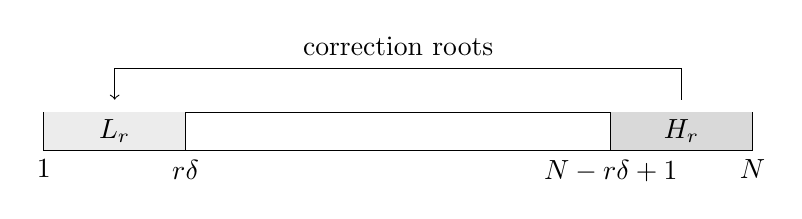
\begin{tikzpicture}[x=0.9cm,y=0.8cm]
 \draw (0,0) rectangle (10,0.6);
 \fill[gray!15] (0,0) rectangle (2,0.6);
 \fill[gray!30] (8,0) rectangle (10,0.6);
 \draw (2,0)--(2,0.6) (8,0)--(8,0.6);
 \node at (1,0.3) {$L_r$};
 \node at (9,0.3) {$H_r$};
 \draw[->] (9,0.8)--(9,1.3)--(1,1.3)--(1,0.8);
 \node at (5,1.65) {correction roots};
 \node[below] at (0,0) {$1$};
 \node[below] at (2,0) {$r\delta$};
 \node[below] at (8,0) {$N-r\delta+1$};
 \node[below] at (10,0) {$N$};
\end{tikzpicture}
\caption{The correction strip goes from the right band
$H_r=\{N-r\delta+1,\ldots,N\}$ to the left band
$L_r=\{1,\ldots,r\delta\}$. Conjugation by one truncated block factor
enlarges each band by at most $\delta$.  Choosing
$N>2(m+1)\delta$ keeps them disjoint throughout the collection.}
\label{kt:strip-figure}
\end{figure}

We claim that conjugating an element of the strip of width
$r\delta$ by one truncated block factor $D_h$, or by its inverse,
keeps it in the strip of width $(r+1)\delta$, whenever $r\leq m$.
It is enough to check a strip root.  Every constituent of $D_h$
goes from an outer index $i$ to a fixed different outer index $j$,
and has inner displacement between $0$ and $d$.  All these
constituents commute.  A constituent initially commuting with the
strip root can therefore be omitted when computing the conjugation:
it also commutes with every conjugate of that root by the other
constituents.

An interacting constituent can change the source endpoint only
when its target is the old source; it then moves that endpoint
left by at most $d$.  It can change the target endpoint only when
its source is the old target; it then moves that endpoint right
by at most $d$.  These assertions, including the coefficients in
their prescribed multiplication order, are precisely the consecutive
Steinberg relations and their reversed versions.  No constituent
can be opposite to a strip root: an edge from its low target to
its high source would have displacement greater than $d$, by the
bound on $N$. This exclusion also holds after one endpoint has moved.
The source inner index minus the target inner index is then greater
than $N-(2r+1)\delta>\delta$, since $r\leq m$ and
$N>2(m+1)\delta$. A constituent of displacement at most $d\leq\delta$
therefore cannot be opposite to an intermediate root.

There is also no accumulation of many shifts at one endpoint during
this single block factor.  After a source change, that source has
outer index $i$, whereas every constituent has target outer index
$j\ne i$, so it cannot change the source again.  After a target
change, that target has outer index $j$, whereas every constituent
has source outer index $i$, so it cannot change the target again.
Both endpoints may change, but each changes at most once.  Every
root produced thus belongs to the strip of width $(r+1)\delta$.
The argument applies to a product of strip roots and to inverse
conjugation as well.  In characteristic two, each block factor is
in fact its own inverse.

Collecting all $D_h$ to the left now gives
\[
 W_v(C_N)=W_v(S_N)\,z,
\]
where $z$ is a product of the wrap factors $F_h$ conjugated by
suffixes of the truncated factors. More explicitly, set
$D_{>h}=D_{h+1}\cdots D_m$ and $D_{>m}=1$. The group identity
\[
 \prod_{h=1}^m(D_hF_h)
 =(D_1\cdots D_m)
   \prod_{h=1}^m(D_{>h}^{-1}F_hD_{>h})
\]
keeps the last product in increasing order of $h$. Thus no correction
factor is used to conjugate another correction. Each suffix has at
most $m$ factors.  The claim puts every resulting correction in the single
strip
\[
 \text{source inner index}>N-(m+1)\delta,
 \qquad
 \text{target inner index}\leq(m+1)\delta.
\]
Its endpoint sets are disjoint by our choice of $N$.  Both evaluated
words have identity matrix image, so $z$ also has identity matrix
image.  Faithfulness of this strip gives $z=1$, as required.
\end{proof}

\subsection{Stable torsion and its descent}

Torsion of nil $K$-groups in positive characteristic is part of the
stable theory
\cite[Corollary~3.3(d)]{Weibel1981}. We make the needed comparison
directly in Steinberg groups and use the rational stability already
proved to descend to the fixed rank.

\begin{proposition}\label{kt:stable-torsion}
Let $n\geq 6$ and $u\in J_n(R)$.  The image of $u$ in
$\St_q(R)$ is torsion for some $q\geq n$ under the standard coordinate
homomorphism.
\end{proposition}

\begin{proof}
Choose a finite root word representing $u$ and apply the grading
homomorphism $\gamma$ to its entries, obtaining the word $u(t)$
from the opening of this section. Its matrix image is the identity,
$u(1)$ represents $u$, and $u(0)$ represents an element of
$J_n(\F_2)$ before the field is included into $R$.

If the word is empty there is nothing to prove.  Otherwise let $m$
be its number of root factors and $d$ the maximum degree of their
entries.  Choose a power of two $N$ with
\[
 N>2(m+1)\max\{1,d\},
\]
and set $W=W_u(C_N)\in\St_{nN}(R)$.

Since $C_N^N=\Id$ and $N$ is a power of two, the binomial identity
in characteristic two gives $(C_N-\Id)^N=0$.  A nilpotent linear
map has an upper triangular matrix with zero diagonal in a basis
adapted to its successive kernels.  Thus some
$P\in\GL_N(\F_2)$ makes $P^{-1}C_NP$ upper triangular with all
diagonal entries equal to $1$.  Lemma~\ref{kt:block-laws} gives
an exact conjugation between the two evaluated root words.  Both
belong to $J_{nN}(R)$, which is central by
Proposition~\ref{prop:centrality}; that conjugation consequently
fixes $W$.  Lemma~\ref{kt:triangular-evaluation} now yields
\[
 W=\prod_{s=1}^{N}\iota_s(u).
\]
Each $\iota_s(u)$ belongs to the central kernel at rank $nN$.
By Lemma~\ref{kt:permutations}, a permutation of coordinates
conjugates any one of these coordinate images to any other.
Centrality therefore makes them equal, and
\begin{equation}\label{kt:cyclic-power}
 W=\iota_1(u)^N.
\end{equation}

On the other hand, Lemma~\ref{kt:wrap-removal} and then
Lemma~\ref{kt:triangular-evaluation}, now with diagonal value $0$,
give
\begin{equation}\label{kt:truncated-power}
 W=W_u(S_N)=\prod_{s=1}^{N}\iota_s(u(0)).
\end{equation}
By Lemma~\ref{kt:field-kernel}, $u(0)$ has finite order.  Its
coordinate images commute, so their product in
\eqref{kt:truncated-power} has finite order as well.  It follows
from \eqref{kt:cyclic-power} that $\iota_1(u)$ has finite order:
if $W^a=1$, then $\iota_1(u)^{Na}=1$.

Finally, a permutation of the $nN$ coordinates carries the ordered
coordinates $(1,1),\ldots,(n,1)$ to the first $n$ usual coordinates.
Lemma~\ref{kt:permutations} identifies $\iota_1(u)$ with a conjugate
of the usual stabilized image of $u$.  Hence that stabilized image
is torsion.  This argument used only coordinate homomorphisms and
never their injectivity.
\end{proof}

\begin{theorem}\label{kt:kernel-torsion}
For every $n\geq 12$, the group $J_n(R)$ is torsion.
\end{theorem}

\begin{proof}
Fix $u\in J_n(R)$ and a homomorphism
$\varphi:J_n(R)\longrightarrow\Q$.  Proposition~\ref{kt:stable-torsion}
provides a rank $q\geq n$ at which the image of $u$ has finite order.
Successively applying Proposition~\ref{prop:rational-stability}
extends $\varphi$ to a homomorphism $J_q(R)\longrightarrow\Q$.
This extension kills the torsion image of $u$, so $\varphi(u)=0$.
The group $J_n(R)$ is abelian by Proposition~\ref{prop:centrality}.
Lemma~\ref{kt:rational-detection} therefore makes $u$ torsion.
Again, no stabilization map was required to be injective.
\end{proof}

\begin{proof}[Proof of Theorem~\ref{thm:main}]
Take the algebra $R$ from Theorem~\ref{thm:algebra} and put
$G=\St_{12}(R)$.  Theorem~\ref{thm:finite-presentation} gives an
ordinary finite presentation of $G$.  Its image $\E_{12}(R)$ is
infinite, because distinct entries in any one elementary matrix
position give distinct matrices and $R$ is infinite.  Thus $G$
is infinite.

By Lemma~\ref{fp:matrix-periodicity}, the elementary matrix group
$\E_{12}(R)$ is periodic.  For $g\in G$, choose a positive integer
$a$ killing its elementary matrix image.  Then $g^a\in J_{12}(R)$,
and Theorem~\ref{kt:kernel-torsion} gives a positive integer $b$
with $(g^a)^b=1$.  Consequently every element of $G$ has finite
order.  The group $G$ is the required infinite, finitely presented
periodic group.
\end{proof}

\subsection{The Kazhdan consequence}\label{sec:kazhdan}

\begin{proof}[Proof of Corollary~\ref{cor:kazhdan}]
Theorem~\ref{thm:algebra} presents \(R\) as a unital associative
\(\F_2\)-algebra on finitely many generators. Since \(\F_2\) is the
prime field, those generators together with \(1\) generate \(R\) as a
ring. Ershov and Jaikin-Zapirain prove that \(\St_n(S)\) has
property~\((T)\) for every finitely generated associative ring \(S\)
with \(1\) and every \(n\geq3\)
\cite[Theorem~6.2]{ErshovJaikinZapirain2010}. This applies directly to
\(S=R\) and \(n=12\). Infinitude, finite presentation, and periodicity
are those of Theorem~\ref{thm:main}.

Write \(G=\St_{12}(R)\). If \(G\) were amenable, normalized
characteristic functions of F\o lner sets would give almost invariant
unit vectors in the left regular representation on \(\ell^2(G)\).
Property~\((T)\) would then give a nonzero invariant vector. Such a
vector is constant on \(G\), and a nonzero constant function on the
infinite group \(G\) is not square-summable. Hence \(G\) is nonamenable.
\end{proof}
